\begin{problem}{넴모넴모}{standard input}{standard output}

네모는 뿌××× 게임에 깊은 감명을 받아 ``넴모넴모'' 게임을 만들었다. 이 게임은 직사각형 모양의 격자판과 ``넴모''라는 수수께끼의 생물을 이용해 하는 아주 간단한 게임이다. 게임의 규칙은 격자판의 비어 있는 칸을 임의로 골라 ``넴모''를 하나 올려놓고, ``넴모''가 올라간 칸 네 개가 $2 \times 2$ 사각형을 이룰 경우 그 위에 있는 ``넴모''들을 모두 없애는 것을 질릴 때까지 반복하는 것이다.

\begin{center}
  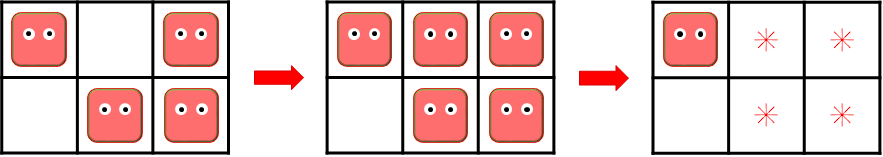
\includegraphics[width=0.7\textwidth]{nemo.png}
\end{center}

하지만 안타깝게도 게임은 정말 재미가 없었고, 네모는 아주 빨리 질려 버리고 말았다. 실망한 네모는 격자판 위에 더 이상 없앨 ``넴모''가 없는 상태에서 게임을 그만두기로 했다. 게임의 결과로 나올 수 있는 상태의 가짓수를 구하여라.

\InputFile
첫 번째 줄에 격자판의 행의 개수 $N$, 열의 개수 $M$($N \ge 1$, $M \ge 1$, $1 \le N \times M \le 25$)이 공백으로 구분되어 주어진다.

\OutputFile
첫 번째 줄에 ``넴모''들이 올라간 칸이 $2 \times 2$ 사각형을 이루지 않도록 격자판에 ``넴모''들을 배치하는 가짓수를 출력한다.

\Example

\begin{example}
\exmp{2 2}{15}%
\exmp{2 3}{57}%
\exmp{3 5}{22077}%
\end{example}

\Notes
$2 \times 2$ 격자판에 ``넴모''들을 안정되게 배치하는 방법은 모든 경우($2^{4}=16$) 중 네 칸 모두에 ``넴모''가 올라가 있는 경우를 제외한 $15$가지가 있다.

\end{problem}
